\section{Experimental results}
\label{sec:benchmarks}

We describe here the implementation of our algorithms and an
application coming from elliptic curve cryptology, isogeny
computation.

\paragraph*{\bf Implementation.} We packaged the algorithms of this
paper in a \texttt{C++} library called \texttt{FAAST} and made it
available under the terms of the \texttt{GNU GPL} software license
from
\mbox{\url{http://www.lix.polytechnique.fr/Labo/Luca.De-Feo/FAAST/}}.

\texttt{FAAST} is implemented on top of the \texttt{NTL}
library~\cite{NTL} which provides the basic univariate polynomial
arithmetic needed here. Our library handles three NTL classes of
finite fields: {\tt GF2} for $p=2$, {\tt zz\_p} for word-size $p$ and
{\tt ZZ\_p} for arbitrary $p$; this choice is made by the user at
compile-time through the use of \texttt{C++} templates and the
resulting code is thus quite efficient.  Optionally, \texttt{NTL} can
be combined with the \texttt{gf2x} package~\cite{gf2x} for better
performance in the $p=2$ case, as we did in our experiments.

All the algorithms of Sections
\ref{sec:fast-tower}--\ref{sec:pseudotrace-frobenius} are faithfully
implemented in \texttt{FAAST}. The algorithms \alg{ApplyIsomorphism}
and \alg{ApplyInverse} have slightly different implementations
\texttt{toUnivariate()} and \texttt{toBivariate()} that allow more
flexibility. Instead of being recursive algorithms doing the change to
and from the multivariate basis $\bB'_i=\{{x_0'}^{e_0}\cdots
{x_i'}^{e_i}\}$, they only implement the change to and from the
bivariate basis $\bD'_i=\{{x_{i-1}}^{e_{i-1}}{x_i'}^{e_i}\}$ with $0\le
e_{i-1}<p^{i-1}d$ and $0\le e_i<p$. Equivalently, this amounts to
switch between the representations
\begin{equation*}
  \wrt\U_i \quad\text{and}\quad
  \wrt\U_{i-1}[X_i']/(X_i'^p-X_i'-\gamma_{i-1}')
  \text{.}
\end{equation*}
The same result as one call to \alg{ApplyIsomorphism} or
\alg{ApplyInverse} can be obtained by $i$ calls to
\texttt{toUnivaraite()} and \texttt{toBivariate()}
respectively. However, in the case where several generic Artin-Schreier
towers, say $(\U_0',\ldots,\U_k')$ and $(\U_0'',\ldots,\U_k'')$, are
built using the algorithms of Section \ref{sec:couveignes-algorithm},
this allows to \emph{mix} the representations by letting the user
chose to switch to any of the bases $\{y_0^{e_0}\cdots y_i^{e_i}\}$
where $y_i$ is either $x_i'$ or $x_i''$. In other words this allows
the user to \emph{zig-zag} in the lattice of finite fields as in
Figure~\ref{fig:lattice}.

\begin{figure}
  \centering
  \begin{equation*}
    \xymatrix@C=1cm{
      & v\wrt\U_k \ar@{<--}@(r,u)[dr] \\
      \U_k'\ar@{-}[r]^{\sigma'} & \U_k\ar@{-}[d] & \U_k''\ar@{-}[l]_{\sigma''} \ar@{--}@(d,u)[dll]\\
      \U_{k-1}'\ar@{-}[r]^{\sigma'} \ar@{--}@(d,u)[drr] & \U_{k-1}\ar@{.}[d] & \U_{k-1}''\ar@{-}[l]_{\sigma''}\\
      \U_1'\ar@{-}[r]^{\sigma'} & \U_1\ar@{-}[d] & \U_1''\ar@{-}[l]_{\sigma''}\ar@{-->}[d]\\
      & \U_0 & *[r]{v\wrt\{{x_0}^{e_0}{x_1''}^{e_1}\cdots {x_{k-1}'}^{e_{k-1}}{x_k''}^{e_k}\}}
    }
  \end{equation*}
  \caption{An example of conversion from the univariate basis to a
    mixed multivariate basis.}
  \label{fig:lattice}
\end{figure}

Besides the algorithms presented in this paper, \texttt{FAAST} also
implements some algorithms described in~\cite{DeFeo10} for minimal
polynomials, evaluation and interpolation, as they are required for the 
isogeny computation algorithm.


\paragraph*{\bf Experimental results.} We compare our timings with
those obtained in Magma~\cite{Magma} for similar questions.  All
results are obtained on an Intel Xeon E5430 (2.6GHz).

\smallskip

The experiments for the \texttt{FAAST} library were only made for the
classes \texttt{GF2} and \texttt{zz\_p}. The class \texttt{ZZ\_p} was
left out because all the primes that can be reasonably handled by our
library fit in one machine-word. In Magma, there exist several ways to
build field extensions:

\begin{description*}
\item [$\bullet$ {\tt quo<U|P>}] builds the quotient of the
  univariate polynomial ring $U$ by  $P \in U$
  (written magma(1) hereafter);

\smallskip

\item [$\bullet$ {\tt ext<k|P>}] builds the extension of the field $k$ by $P \in
  k[X]$ (written magma(2));

\smallskip

\item [$\bullet$ {\tt ext<k|p>}] builds an extension of degree $p$ of $k$
  (written mag\-ma(3)).
\end{description*}

\smallskip\noindent We made experiments for each of these choices where this makes sense.


\smallskip The parameters to our algorithms are
$(p,d,k)$. Thus, our experiments describe the following situations:

\begin{itemize}
\item {\em Increasing the height $k$.} Here we take $p=2$ and $d=1$ (that is,
  $\U_0=\F_2$); the $x$-coordinate gives the number of levels we
  construct and the $y$-coordinate gives timings in seconds, in {\em
    logarithmic} scale.

  This is done in Figure~\ref{fig:height}. We let the height of the
  tower increase and we give timings for (1) building the tower of
  Section~\ref{sec:fast-tower} and (2) computing an isomorphism with a
  random arbitrary tower as in Section~\ref{sec:couveignes-algorithm}.
  In the latter experiment, only the magma(2) approach was meaningful
  for Magma.

\smallskip

\item {\em Increasing the degree $d$ of $\U_0$.} Here we take $p=5$
  and we construct $2$ levels; the $x$-coordinate gives the degree $d
  = [\U_0:\F_p]$ and the $y$-coordinate gives timings in seconds.
  This is done in Figure~\ref{fig:p-d} (left).


  \smallskip

\item {\em Increasing $p$.} Here we take $d=1$ (thus $\U_0=\F_p$) and
  we construct $2$ levels; the $x$-coordinate gives the characteristic
  $p$ and the $y$-coordinate gives timings in seconds.  This is done
  in Figure~\ref{fig:p-d} (right).

\end{itemize}

\smallskip 

\begin{figure}
  \centering
%  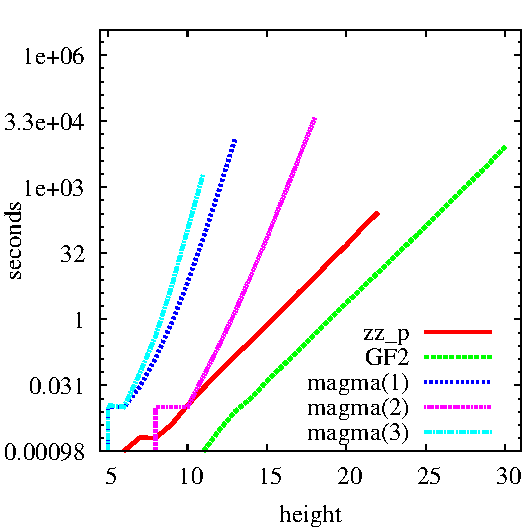
\includegraphics[height=0.5\textwidth]{build1}
%  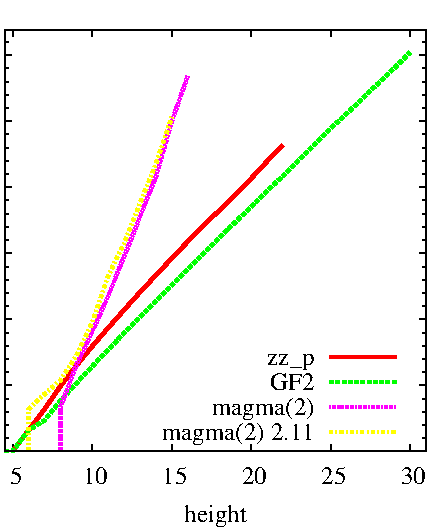
\includegraphics[height=0.5\textwidth]{iso1}
  
  \caption{Build time (left) and isomorphism time (right) with respect to tower height. Plot is in logarithmic scale.}
  \label{fig:height}
\end{figure}

\begin{figure}
  \centering
%  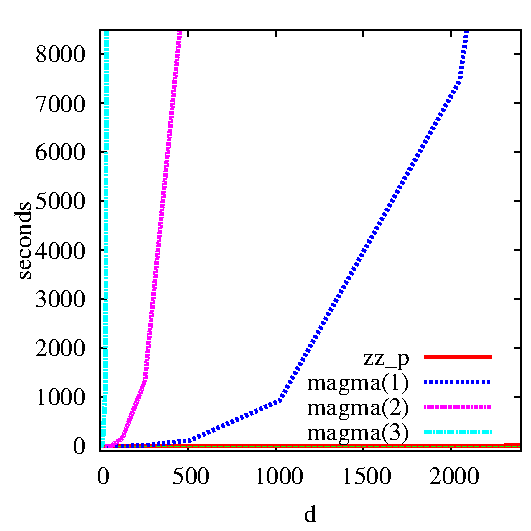
\includegraphics[height=0.5\textwidth]{build-d}
%  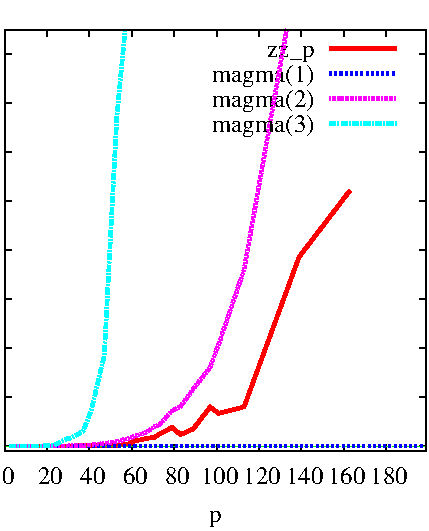
\includegraphics[height=0.5\textwidth]{build-p}
  
  \caption{Build times with respect to $d$ (left) and $p$ (right).}
  \label{fig:p-d}
\end{figure}

The timings of our code are significantly better for increasing height
or increasing $d$. Not surprisingly, for increasing $p$, the magma(1)
approach performs better than any other: the {\tt quo} operation
simply creates a residue class ring, regardless of the
(ir)reducibility of the modulus, so the timing for building two levels
barely depend on $p$. Yet, we notice that \texttt{FAAST} has
reasonable performances for characteristics up to about $p=50$.

\smallskip

In Tables~\ref{tab:arith-gf2} and~\ref{tab:arith-zzp} we provide some
comparative timings for the different arithmetic operations provided
by \texttt{FAAST}. The column ``Primitive'' gives the time taken to
build one level of the primitive tower (this includes the
precomputation of the data as described in
Subsection~\ref{sec:level-embedding:lift-up}); the other entries are
self-explanatory. Product and inversion are just wrappers around
\texttt{NTL} routines: in these operations we didn't observe any
overhead compared to the native \texttt{NTL} code. All the operations
stay within a factor of $30$ of the cost of multiplication, which is
satisfactory.

\begin{table}
  \centering
  \begin{tabular}{l | r | r | r | r | r | r | r}
    level & Primitive & Push-d. & Lift-up & Product & Inverse & apply $\sigma^{-1}$ & apply $\sigma$ \\
    \hline
     19 &  1.061 & 0.269 &  1.165 & 0.038 &  0.599 &  0.572 &  1.152\\
     20 &  2.381 & 0.538 &  2.554 & 0.076 &  1.430 &  1.146 &  2.333\\
     21 &  5.284 & 1.083 &  5.645 & 0.171 &  3.331 &  2.306 &  4.807\\
     22 & 11.747 & 2.202 & 12.595 & 0.430 &  7.730 &  4.811 & 10.051\\
     23 & 26.441 & 4.654 & 28.641 & 0.961 & 18.059 & 10.240 & 21.494\\
  \end{tabular}
  \caption{Some timings in seconds for arithmetics in a generic tower built over $\F_2$ using \texttt{GF2}.}
  \label{tab:arith-gf2}
\end{table}

\begin{table}
  \centering
  \begin{tabular}{l | r | r | r | r | r | r | r}
    level & Primitive & Push-d. & Lift-up & Product & Inverse & apply $\sigma^{-1}$ & apply $\sigma$ \\
    \hline
    18 &   9.159 &  0.514 &   8.278 &  0.321 &   6.432 &  2.379 &   6.624\\
    19 &  21.695 &  1.130 &  20.388 &  1.083 &  14.929 &  6.289 &  18.202\\
    20 &  49.137 &  3.058 &  48.605 &  2.444 &  33.986 & 10.716 &  32.493\\
    21 & 122.252 &  7.476 & 123.369 &  5.307 &  92.827 & 26.437 &  76.780\\
    22 & 275.110 & 15.832 & 279.338 & 10.971 & 210.680 & 47.956 & 134.167\\
  \end{tabular}
  \caption{Some timings in seconds for arithmetics in a generic tower built over $\F_2$ using \texttt{zz\_p}.}
  \label{tab:arith-zzp}
\end{table}


Finally, we mention the cost of precomputation. The precomputation of
the images of $\sigma$ as explained in
Section~\ref{sec:couveignes-algorithm} is quite expensive;
most of it is spent computing pseudotraces. Indeed it took one week to
precompute the data in Figure~\ref{fig:height} (right), while all the
other data can be computed in a few hours. There is still space for
some minor improvement in \texttt{FAAST}, mainly tweaking recursion
thresholds and implementing better algorithms for small and moderate
input sizes. Still, we think that only a major algorithmic improvement
could consistently speed up this phase.


\paragraph*{\bf Isogeny algorithm.} An isogeny is a regular map
between two elliptic curves $\mathscr{E}$ and $\mathscr{E}'$ that is
also a group morphism.  In cryptology, isogenies are used in the
Schoof-Elkies-Atkin point-counting algorithm~\cite{BlSeSm99}, but also
in more recent constructions~\cite{RoSt06,Teske06}, and the fast
computation of isogenies remains a difficult challenge.

Our interest here is Couveignes' isogeny
algorithm~\cite{Couveignes96}, which computes isogenies of degree
$\sim p^k$; the algorithm relies on the interpolation of a rational
function at special points in an Artin-Schreier tower. The original
algorithm in~\cite{Couveignes96} was first implemented
in~\cite{Lercier97}; Couveignes' later paper~\cite{Couveignes00}
described improvements to speed up the computation, but as we already
mentioned, a key component, fast arithmetic in Artin-Schreier towers,
was still missing. The recent paper~\cite{DeFeo10} combines this
paper's algorithms and other improvements to achieve a completely
explicit version of~\cite{Couveignes00}.

\begin{figure}
  \centering
%  \includegraphics[width=0.9\linewidth]{couveignesII}

  \caption{Timings for the isogeny algorithm. Isogenies of degree
    increasing degree are computed between curves defined over
    $\F_{2^{101}}$.}
  \label{fig:couveignes}
\end{figure}

The algorithm is composed of 5 phases:
\begin{enumerate}
\item Depending on the degree $\ell$ of the isogeny to be computed, a
  parameter $k$ is chosen such that $p^{k-1}(p-1)>4\ell-2$;
\item\label{alg:cou:pri} a primitive tower of height $\sim k$ is
  computed (the precise height depends on $\mathscr{E}$ and
  $\mathscr{E'}$, in the example of figure~\ref{fig:couveignes} it is
  always equal to $k-2$);
\item\label{alg:cou:E} an Artin-Schreier tower in which the
  $p^k$-torsion points of $\mathscr{E}$ are defined is computed and an
  isomorphism is constructed to the primitive tower;
\item\label{alg:cou:E'} an Artin-Schreier tower in which the
  $p^k$-torsion points of $\mathscr{E'}$ are defined is computed and
  an isomorphism is constructed to the primitive tower;
\item\label{alg:cou:int} a mapping from $\mathscr{E}[p^k]$ to
  $\mathscr{E'}[p^k]$ is computed through interpolation;
\item\label{alg:cou:loop} all the possible mappings from
  $\mathscr{E}[p^k]$ to $\mathscr{E'}[p^k]$ are computed through
  modular composition until one is found that yields an isogeny.
\end{enumerate}

We ran experiments for curves defined over the base field
$\F_{2^{101}}$ for increasing isogeny degree. Figure
\ref{fig:couveignes} shows the timings for two implementations
of~\cite{DeFeo10} based on \texttt{FAAST} and one implementation of
the same algorithm based on the magma(2) approach; remark that the
time scale is logarithmic. The running time is probabilistic because
step~\ref{alg:cou:loop} stops as soon as it has found an isogeny; we
plot the average running times with bars around them for
minimum/maximum times; the distribution is uniform. Note that the plot
in the original ISSAC '09 version of this paper shows timings that are
one order of magnitude worse. This was due to a bug that has later
been fixed.

\begin{table}
  \centering
  \begin{tabular}{l | r | r | r | r | r | r}
    degree & step~\ref{alg:cou:pri} & step~\ref{alg:cou:E} & step~\ref{alg:cou:int} & \multicolumn{3}{|c}{step~\ref{alg:cou:loop}} \\
    &&&&preconditioning & avg \# iterations & iteration\\
    \hline
    3 & 0.008 & 0.053 & 0.124 & 0.005 & 8 & 0\\
    5 & 0.004 & 0.161 & 0.310 & 0.019 & 16 & 0.002\\ 
    11 & 0.008 & 0.469 & 0.749 & 0.096 & 32 & 0.001\\
    17 & 0.014 & 1.312 & 1.779 & 0.227 & 64 & 0.003\\
    37 & 0.039 & 3.544 & 4.168 & 1.130 & 128 & 0.013\\
    67 & 0.078 & 9.306 & 9.651 & 6.107 & 256 & 0.052\\
    131 & 0.189 & 23.79 & 22.124 & 34.652 & 512 & 0.207\\
    257 & 0.383 & 59.82 & 50.532 & 200.980 & 1024 & 0.812\\
  \end{tabular}
  \caption{Comparative timings for each phase of the isogeny algorithm using \texttt{GF2}.}
  \label{tab:couveignes}
\end{table}

Table~\ref{tab:couveignes} shows comparative timings for each phase of
the algorithm.  The reason why we left step~\ref{alg:cou:E'} out of
the table is that it is essentially the same as step~\ref{alg:cou:E}
and timings are nearly identical. Step~\ref{alg:cou:loop} is
asymptotically the most expensive one; it uses some preconditioning to
speed up each iteration of the loop. From the point of view of this
paper, the most interesting steps
are~\ref{alg:cou:pri}-\ref{alg:cou:int} since they are the only ones
that make use of the library \texttt{FAAST}.

For $p=2$, it should be noted that Lercier's isogeny
algorithm~\cite{Lercier96} has better performance; for generic, small,
$p$ we mention as well a new algorithm by Lercier and
Sirvent~\cite{LeSi09}. See~\cite{DeFeo10} for further discussions on
isogeny computation.



% Local Variables: 
% mode:flyspell
% ispell-local-dictionary:"american"
% TeX-master: "../these"
% mode: Tex-PDF
% mode: reftex
% End: 
%
% LocalWords:  univariate isogeny Couveignes isogenies Artin Schreier
